\chapter{Background Research}
\label{chapter2}

\section{Problem Overview}
Compute power of games can be offloaded to a server of much powerful computers and then streamed to a client with lower specification hardware such as a laptop or a mobile device. With this comes risks and shortcomings that need to be factored. One of these problems are the latency of the game. Latency can be huge factor in the gameplay such as high-paced games like first-person shooters or fighting games. The delay in pressing a button on the gamepad to seeing the action performed on the screen needs to be kept to a minimum. This idea of interaction delay tolerance being different from genre to genre of games is discussed by Shea et al. \cite{shea2013cloud}. As stated above, a player of FPS games can only tolerate the least which is around 100ms whereas Role playing game (RPG) gamers can tolerate around 500 ms.
\newline
\par
Another problem that is directly linked to delay in the system is the effect of packet loss. As stated in the \textit{Eight Fallacies of Distributed Computing} \cite{deutsch1994eight}, it should be assumed that latency is never zero as mentioned above as well as network is not always reliable. This means that packet loss can occur which in terms of cloud computing can mean the degradation of image quality. In the investigation conducted by Jarschel et al. \cite{jarschel2011evaluation} in which they surveyed average consumers about the importance of packet loss and delay. Generally the quality of the video streamed to the clients plays an important role as the participants were open to using such as a service if provided in good quality.

\section{Cloud Computing}
According to the National Institute of Standards and Technology \cite{mell2011nist}, cloud computing is a means of providing on demand access to computing resources over the network. This should be executed with minimal management effort or service provider interaction

\section{Cloud Gaming}
Cloud gaming is new technology that can be seen as an alternative by having the games run remotely on a server and then streamed to the user. Performing computations remotely as with streaming games remotely is believed to gain traction in the future in the same way how streaming videos and audio have become ubiquitous through services such as Netflix and Spotify. NVIDIA's GRID Cloud Gaming advancements have shown that this is becoming the case. As stated by Mariano in \textit{Is cloud gaming the future of the gaming industry} \cite{mariano2015cloud}, cloud gaming is increasingly becoming an attractive option for consumers as higher end games can then work on simpler, cheaper clients as well as with devices that they may already own also known as thin clients.
\newline
\par
These thin clients are responsible for displaying the game frames rendered on the cloud server side in the form of video frames. Also, it has to collect and process the game control inputs from the user and send these to cloud to be registered as inputs on the game engine. According to Shea et al \cite{shea2013cloud}, cloud gaming would be of great benefit to the game industry as it would open the user base to the thin clients. For example the recommended specifications to run the 2015 Game of the Year title Witcher 3\cite{goty2015} would require a system that has \cite{witcher}:
\begin{itemize}
 \item CPU: Intel Core i7 3770 3.4 GHz / AMD FX-8350 4 GHz
 \item GPU: GeForce GTX 770 / AMD Radeon R9 290
 \item RAM: 8GB
\end{itemize}
A system that has these components would cost around \textlira400 and this does not include peripherals such as keyboard, mouse and monitor. The latest tablets and laptops can barely if at all meet the recommended specifications to run the game natively. Furthermore, games will have to deal with running on different hardware architectures and operating systems. Cloud gaming would enable consumers with lower end devices to run and play graphically intensive games.
\newline
\par
In the paper \textit{Cloud Gaming: A Green Solution to Massive Multiplayer Online Games} \cite{chuah2014cloud} it mentions that NVIDIA has introduced SHIELD which is a mobile gaming device that can be connected to a desktop PC with a compatible NVIDIA GPU and stream gameplay to the device via 802.11n WiFi. Another feature is the ability to connect to one of NVIDIA's data centres to play games from their selection of stream-ready games. One of the benefits of this service is the convenience of not having to wait for the download and installation of the game as you simply pick a game and instantly start playing. The service also boasts gameplay performance of up to 1080p at 60fps which are deemed by gamers to be the target performance.

\clearpage
\begin{figure}
 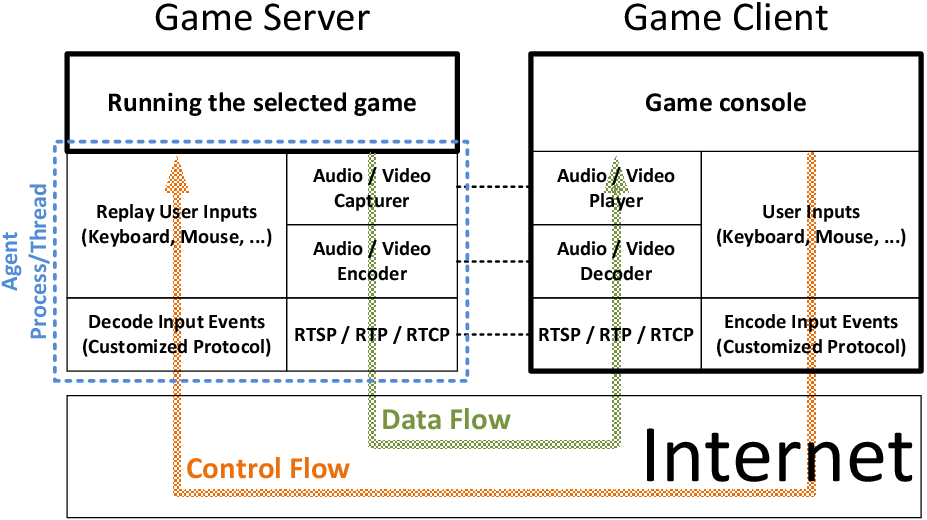
\includegraphics[width=\linewidth]{images/arch.png}
 \caption{Cloud gaming system architecture}
 \label{fig:arch}
\end{figure}

A simple cloud gaming architecture consists of several procedures which adds on top of the game engine process as shown in Figure \ref{fig:arch}. The client would send user inputs through some form of controller like a keyboard, mouse, or gamepead to the thin client. The game client then encodes these commands so it can easily be sent to the game server via network. When the server receives the user inputs, it simulates them so the game that is running recognises them. The game renders the frames produced as a result of the inputs and are captured and encoded to video frames. This is done so it can be easily streamed to the client through the use of Real Time Streaming Protocol (RTSP) which is a network control protocol that manages delivery of data with real time properties \cite{rtsp}. The thin client uses RTSP to receive the video frames and decodes them to be displayed on a video player. The user then sees the results of the button presses sent from the game running on the server side. 
\par
Due to the many different processes involved in the architecture of a cloud gaming system, managing latency has become a problem. A traditional gaming system already experiences latency and as shown in Figure \ref{fig:latency}, this arises from the game pipeline and display lag. The game pipiline latency is the amount of time it takes for the game to comput and render a frame and the display lag is the time it takes to display the frames on the screen. Display lag can be caused by display's scaler since current display's have a fixed resolution and expensive image processing such as dynamic contrast and motion interpolation \cite{displaylag}. Cloud gaming introduces latency from capturing/encoding game frame to video frame, network and decoding on the client side.

\begin{figure}[h]
 \centering
 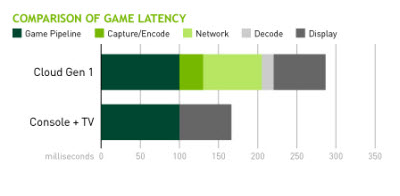
\includegraphics[width=0.7\linewidth]{images/latency.png}
 \caption{Latency in cloud gaming}
 \label{fig:latency}
\end{figure}

\section{Latency Mitigation}
One method of latency mitigation is to simply move the server to the clients. This means that traffic will have to travel less distance therefore latency will decrease. Unfortunately, this solution is not feasible since building and maintaining data centres are expensive. Video streaming services such as Netflix and YouTube use buffering which loads video data before playing the video in order for continuous playback. This cannot be done for live cloud gaming so other solutions to improve experiences of latency sensitive games must be explored.

\subsection{Software-Defined Networking}
As stated by Kirkpatrick \cite{kirkpatrick2013software}, software-defined networking (SDN) is a new networking architecture that allows programmers to quickly reconfigure and define network usage. Whilst signifcant advances have been in other areas of technology, networking has not been able to evolve in the same pace.
\newline
\par
Similar to mobile phones shifting to the world of smartphones with the help of APIs (application program interface), in an SDN environment, applications can communicate with network switches through an API. The API can be used to quickly reconfigure the resources of the network to accommodate the needs of the applications being executed. This main benefit of using SDN is also discussed in \textit{Improving network management with software defined networking} \cite{kim2013improving}. Kim et al mentions that network operators will not need to configure all the network devices indivdually to make network behaviour changes, but instead make network-wide traffic forwarding decisions. The SDN controller is used for this and would have global knowledge of the state of the network.
\newline
\par
SDN consists of two planes, the data and control plane. The data plane also known as the forwarding plane is the part of the network that carries user traffic by forwarding them to the next hop along the path to its destination in accordance to the logic in the control plane. The control plane has command where the traffic is sent by creating the routing tables and is also repsonsible for managing connections between switches, handling errors and exceptions.

\subsection{Speculative Execution: Outatime}
Another form of latency mitigation that is being explored is Microsoft's Outatime which uses \textit{speculation to enable low-latency continuous interaction for mobile cloud gaming} \cite{lee2015outatime}.
\newline 
\par
Outatime basically predicts multiple possible frame outputs that may appear in the future of the game's render scene on the client side. It has to predict what frames may be needed at least a full end host round trip time (RTT) ahead of time the client actually produces game input controls.
\newline
\par
Outatime was extensively tested

\section{Related Works}
\lipsum[1-1]